%%%%%%%%%%%%%%%%%%%%%%%%%%%%%%%%%%%%%%%%%
% Plasmati Graduate CV
% LaTeX Template
% Version 1.0 (24/3/13)
%
% This template has been downloaded from:
% http://www.LaTeXTemplates.com
%
% Original author:
% Alessandro Plasmati (alessandro.plasmati@gmail.com)
%
% License:
% CC BY-NC-SA 3.0 (http://creativecommons.org/licenses/by-nc-sa/3.0/)
%
% Important note:
% This template needs to be compiled with XeLaTeX.
% The main document font is called Fontin and can be downloaded for free
% from here: http://www.exljbris.com/fontin.html
%
%%%%%%%%%%%%%%%%%%%%%%%%%%%%%%%%%%%%%%%%%

%----------------------------------------------------------------------------------------
%	PACKAGES AND OTHER DOCUMENT CONFIGURATIONS
%----------------------------------------------------------------------------------------

\documentclass[a4paper,10pt]{article} % Default font size and paper size

\usepackage{fontspec} % For loading fonts
\defaultfontfeatures{Mapping=tex-text}
\setmainfont[SmallCapsFont = Fontin SmallCaps]{Fontin} % Main document font

\usepackage{xunicode,xltxtra,url,parskip} % Formatting packages

\usepackage[usenames,dvipsnames]{xcolor} % Required for specifying custom colors


\usepackage[big]{layaureo} % Margin formatting of the A4 page, an alternative to layaureo can be \usepackage{fullpage}
% To reduce the height of the top margin uncomment: \addtolength{\voffset}{-1.3cm}

\usepackage{hyperref} % Required for adding links	and customizing them
\definecolor{linkcolour}{rgb}{0,0.2,0.6} % Link color
\hypersetup{colorlinks,breaklinks,urlcolor=linkcolour,linkcolor=linkcolour} % Set link colors throughout the document

\usepackage{titlesec} % Used to customize the \section command
\titleformat{\section}{\Large\scshape\raggedright}{}{0em}{}[\titlerule] % Text formatting of sections
\titlespacing{\section}{0pt}{3pt}{3pt} % Spacing around sections


\usepackage[spanish]{babel} 
\usepackage[latin1]{inputenc} 

\begin{document}

\pagestyle{empty} % Removes page numbering

\font\fb=''[cmr10]'' % Change the font of the \LaTeX command under the skills section

%----------------------------------------------------------------------------------------
%	NAME AND CONTACT INFORMATION
%----------------------------------------------------------------------------------------

\par{\centering{\Huge Juan \textsc{Hernández García}}\bigskip\par} % Your name

\section{Personal Information}

\noindent\begin{minipage}{0.3\textwidth}% adapt widths of minipages to your needs
\begin{tabular}{rl}
\textsc{DNI:} & 23297156L \\
\textsc{Birthdate:} & 13 Julio 1990 \\
\textsc{Address:} & St/La Seda, N7, 2E, Lorca (Murcia) \\
\textsc{Phone:} & 617117423\\
\textsc{email:} & \href{mailto:juanhgw@gmail.com}{juanhgw@gmail.com} \\
\textsc{Linkedin:} & \url{https://es.linkedin.com/in/juansoftwareengineer} \\
\textsc{GitHub:} & \url{https://github.com/juanhg}
\end{tabular}
\end{minipage}%
\hfill%
\begin{minipage}{0.6\textwidth}\raggedleft
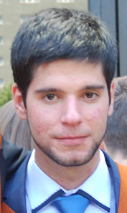
\includegraphics[width=24mm, height=37mm]{pictures/photo2}
\end{minipage}

%----------------------------------------------------------------------------------------
%	WORK EXPERIENCE 
%----------------------------------------------------------------------------------------



\section{Experience}

\begin{tabular}{r|p{11cm}}

\textsc{April 2015} & \textbf{Software Engineer} \\
\textsc{November 2014} & \emph{Tourapp}\\
& \footnotesize{Principal Software Engineer in an image restoration software for
mobile devices that uses the integrated information of the sensors
(gyroscope, magnetometer, accelerometer, etc).}  \\
\multicolumn{2}{c}{} \\

\textsc{November 2014} & \textbf{Freelance Software Engineer} \\
\textsc{July 2014} & \emph{Tertius Informática SL}\\
& \footnotesize{Devolpment of complete application modules of a
business software, in close collaboration with the free software foundation,
\textit{Fidesol}.}\\
\multicolumn{2}{c}{} \\

\textsc{Today} & \textbf{Founder} \\
\textsc{March 2014} & \emph{Nik Nak Studio}\\
& \footnotesize{Founder and Principal Software Engineer at Nik Nak Studio,  a
design studio focused on all things interactive: a graphic design and web 
development studio with a focus on interaction design and user experience.}\\
\textsc{Website} & \url{www.niknak.es} \\
\multicolumn{2}{c}{} \\

\textsc{June 2014} & \textbf{Software Engineer} \\
\textsc{November 2013} & \emph{University of Granada}\\
& \footnotesize{Development and design of physical simulation models.}\\
\multicolumn{2}{c}{} \\

\textsc{July 2014} & \textbf{Research Engineer} \\
\textsc{November 2013} & \emph{University of Granada}\\
& \footnotesize{Research in Neuroscience, programming Brain-Computer
Intefaces.}\\
\multicolumn{2}{c}{} \\

\end{tabular}

\section{Technical Skills}

\begin{tabular}{r|p{11cm}}
\textsc{\textbf{Development}} & Test Driven Development (TDD) \\
\textsc{\textbf{Methodologies}} &  Clean Code Methodology\\
& Scrum (Only applied on academic enviroment) \\
\multicolumn{2}{c}{} \\

\textsc{Programming} & \textsc{Android}, \textsc{Java}, \textsc{C\#},
\textsc{C++}, \textsc{C} \\
\textsc{Languages} &  \textsc{HTML}, \textsc{PHP}, {\fb \LaTeX}\setmainfont[SmallCapsFont=Fontin
SmallCaps]{Fontin-Regular}\ldots  \\
\multicolumn{2}{c}{} \\

\textsc{IDEs} & \textsc{Visual Studio}, \textsc{Eclipse}, \textsc{Android
Studio}, \textsc{NetBeans}\ldots. \\
\multicolumn{2}{c}{} \\

\textsc{Version Control} & \textsc{GitHub}, \textsc{Bitbucket}\ldots
\\
\multicolumn{2}{c}{} \\
\end{tabular}


%----------------------------------------------------------------------------------------
%	EDUCATION
%----------------------------------------------------------------------------------------

\section{Education}

\begin{tabular}{r|p{11cm}}

\textsc{Currently} & \textbf{Master of Data Science and Computer Engineering} \\
\textsc{(Almost finished)} & \emph{Computer Engineering
Specialization}\\
& \emph{University of Granada} \\
\multicolumn{2}{c}{} \\

\textsc{July} 2014 & \textbf{Computer Engineering} \\
 & \emph{University of Granada}\\ 
 Final Project & Compiler and specific language for prototyping and musical
generation.\\ 
Honor Mentions & Final Project, Programming Methodology, Data Structures,
Semantic and Programming Languages, Theory of the Information and Communication, Language
Processors, Advanced Database Models, etc.\\
\multicolumn{2}{c}{} \\

\textsc{May} 2013 & \textbf{Mobile applications development with ANDROID
devices}\\
\textsc{Duration} & 120 hours \\
\multicolumn{2}{c}{} \\

\textsc{February} 2012 & \textbf{Real configuration scenarios of CISCO routers
and switches}\\
\textsc{Duration} & 40 hours \\
\multicolumn{2}{c}{} \\

\textsc{March} 2010 & \textbf{Web 2.0: Architecture oriented to services in
JAVA}\\
\textsc{Duration} & 50 hours\\
\multicolumn{2}{c}{} \\
\end{tabular}

\section{References}

\begin{tabular}{p{146mm}}

\textbf{Modesto Torcuato López López} \\
\emph{Ph.D. in Physics, University of Granada}\\ \\
Juan Hernández García has develop his job in an exceptional way. I can affirm
too, that shows wonderful abilities, dedication, knowledge, and job commitment.
I want to highlight the fact that his participation has been essential to the
development and completion of the innovation project 13-46. \\
\multicolumn{1}{c}{}
\end{tabular}

%----------------------------------------------------------------------------------------
%	LANGUAGES
%----------------------------------------------------------------------------------------

\section{Languages}

\begin{tabular}{r|p{11cm}}
\textsc{English} & B2\\
\textsc{French} & Basic level\\
\textsc{Spanish} & Native language\\
\end{tabular}

%----------------------------------------------------------------------------------------
%	INTERESTS AND ACTIVITIES
%----------------------------------------------------------------------------------------

\section{Interests and Activities}

\begin{itemize}
  \item Videogames development
  \item Bio-Technology
  \item Neural computation
  \item Web design
  \item Literature and current poetry
  \item Rock vocalist
  \item Handball player (until 2010)
\end{itemize}
%----------------------------------------------------------------------------------------

\end{document}
